\documentclass[12pt,a4paper]{article}
\usepackage[utf8]{inputenc} 
\usepackage{latexsym,amssymb,amsmath}
%\usepackage{xltxtra} % charge aussi fontspec et xunicode,
                     % nécessaires...
% \usepackage[latin1]{inputenc}
\usepackage[T1]{fontenc}
\usepackage[francais]{babel}

\usepackage{listings} \lstset{language=C, showstringspaces=false}
\usepackage{graphicx}
\usepackage{pst-tree}

\topmargin -1cm 
\oddsidemargin -10mm 
%\evensidemargin 0mm 
\textheight 27cm 
\textwidth 18cm 
\columnsep 4.1mm

\parindent 1.0em 
\headsep 0mm 
\headheight 0pt 
\lineskip 0pt
\parskip 1em

\normallineskip 0pt 
\def\baselinestretch{1}

\sloppy \hbadness=10000

% arbres
\newcommand{\n}[2]{
  \pstree{\Tr{#1}}{#2}}
\newcommand{\f}[1]{\TR{#1}}
\newcommand{\x}[1]{\pstree[linestyle=none,arrows=-,levelsep=1ex]
  {\Tfan}{\f{#1}}}
\psset{treemode=R,levelsep=20ex,treesep=1em,nodesep=1em}


\begin{document}
\newcommand{\entete}[1]{
        \noindent
        \rule{\linewidth}{0.5mm}\\
        \noindent
        Universit\'e Paris-Nord \hfill CP2I 1\\
        \noindent
        Institut Galil\'ee \hfill Ann\'ee 2008-2009\\
        Eléments d'Informatique - $1^{\text{er}}$ semestre
        \begin{center} {\bf\Large {#1}}
        \end{center}
        \rule{\linewidth}{0.5mm}
}

\entete{Présentation de Linux et KDE}

\newcommand{\puis}{\ensuremath{\rightarrow\ }}


\paragraph{Objectif de TP :\\}

Familiarisation avec l'environnement KDE, le système de fichier Linux et la manipulation du
gestionnaire de fichiers (Konqueror).


\section{SYSTÈME D'EXPLOITATION : INTRODUCTION À LINUX (UNIX)}
\subsection{Multiboot : Grub}

   La séquence de boot (démarrage en français) se décompose ainsi sur
   un PC~:

   \begin{itemize}
   \item {\bf BIOS} (Basic Input Output System) programme résident en
     mémoire morte, vérifiant la mémoire, la présence des
     périphériques de stockage (le rôle plus général du BIOS est de
     configurer les différents paramètres de la carte mère). Au
     démarrage, le BIOS (d'après sa configuration) choisit le
     périphérique contenant le système d'exploitation à démarrer~;

   \item {\bf GRUB} permet de choisir un système à démarrer parmi
     d'autres, ici Windows ou Linux.
   \end{itemize}


   \paragraph{Pour utiliser GRUB :\\}
   

   \begin{enumerate}
   \item guetter l'apparition de l'écran graphique pendant le
     démarrage de la machine ;


   \item à l'aide des flèches, sélectionner le système choisi (ici,
     Linux).


   \item Appuyer sur la touche entrée : l'ordinateur démarre alors
     sous le système choisi.
   \end{enumerate}


 \subsection{Connection de l'utilisateur}

   Le système démarre et il vous est proposé un écran vous permettant
   de vous connecter, en d'autres termes d'endosser l'identité d'un
   utilisateur de Linux. Le système étant basé sur le principe du
   multi-utilisateurs, vous devez obligatoirement endosser une
   identité pour pouvoir utiliser les ressources du système. 

   Après s'être identifié sous linux, deux modes sont possibles : le
   mode console (texte), et le mode graphique (avec des fenêtres).

   Par défaut, il y a 6 consoles et un mode graphique. Pour aller du
   mode graphique à la console, taper CTRL+ALT+Fi où i varie de 1 à
   6. Pour repasser en mode graphique, taper ALT+F7. Pour passer d'une
   console à l'autre, taper ALT+Fi où i est la console où vous désirez
   aller.    Nous allons pour le moment nous connecter en mode
   graphique.

   Commencez par cliquer sur le bouton {\tt Session}, et cochez la
   case {\tt KDE} dans la fenêtre qui apparaît, et validez votre
   choix.

   Pour ce premier TP, entrez ensuite l'identité ({\bf login}),
   puis le mot de passe ({\bf password}) qu'on vous a assignés.
   Vous remarquerez que le mot de passe ne s'affiche
   pas en clair, pour éviter qu'on ne lise par dessus votre épaule.



\section{KDE : PREMIÈRES MANIPULATIONS}

KDE est un gestionnaire de fenêtre (« window manager » en VO) qui fournit une interface
graphique conviviale (à la Windows ou MacOS). À la différence de Windows et MacOS, KDE
fournit d'office un gestionnaire de bureaux.

\subsection{Gestion des bureaux}

\subsubsection{Présentation}
 
Un \emph{bureau} est un \emph{espace de travail}. KDE dispose de
deux ou quatre bureaux initiaux mais il est possible de définir jusqu'à seize
bureaux à la fois. 

Pour se déplacer d'un bureau à un autre, on peut utiliser les
icônes situées sur le panneau de contrôle (barre du bas d'écran) ou
la combinaison des touches Crtl+F2 pour accéder au deuxième bureau,
Ctrl+F3 pour le troisième bureau, etc. 

Par défaut, le bureau de KDE se présente de la façon suivante~:

\begin{itemize}
\item en bas, le {\bf tableau de bord}~: c'est une barre rassemblant
  des menus pour accéder aux applications, des icônes permettant de
  lancer directement certaines applications et une zone permettant de
  visualiser les applications en cours~;
  
\item au centre, l'espace de travail proprement dit (c'est à dire le
  bureau).
\end{itemize}


\subsubsection{ Bulles d'aide}
Si l'utilisateur déplace la souris sur une icône et la laisse immobile
quelques instants, une \emph{bulle d'aide} s'affiche et indique à
l'utilisateur le nom et une description sommaire de l'application
correspondante. 


\subsubsection{Icônes du bureau}
   Le bureau est constitué d'icônes de travail (qui représentent
   généralement des raccourcis pour accéder à des répertoires ou des
   applications). Repérez les icônes \emph{Dossier personnel} et
   \emph{Corbeille}, qui seront utiles pour la suite du TP.



\subsubsection{Le tableau de bord}
    Le tableau de bord sert à lancer rapidement certaines
    applications, à passer d'un bureau à un autre, mais aussi à avoir
    accès à l'ensemble des applications disponibles sous KDE à l'aide
    du menu principal.

    Exploration de quelques icônes du tableau (en partant de la
    gauche)~:

    \begin{itemize}
    \item le bouton {\bf Cacher/Montrer} : flèche étroite située aux deux
      extrémités du panneau. En cliquant dessus, le panneau est masqué
      (pour libérer de l'espace de travail).

    \item le {\bf menu principal} (icône K, étoile, chapeau rouge ou
      spirale selon les distributions Linux)~: ce menu permet
      d'accéder rapidement aux applications et fonctionnalité de KDE,
      via des sous-menus. C'est l'équivalent du menu {\emph{Démarrer}}
      de Windows.

    \item icône {\bf liste des fenêtres} (liste des applications actives)~:
      affiche la liste des bureaux, et les applications ouvertes dans
      chaque bureau. Vous pouvez utiliser cette liste pour passer d'un
      bureau à un autre, d'une application à une autre.

    \item les autres icônes sont laissées à la découverte de
      l'utilisateur (on peut utiliser pour cela les bulles d'aide).

    \end{itemize}


    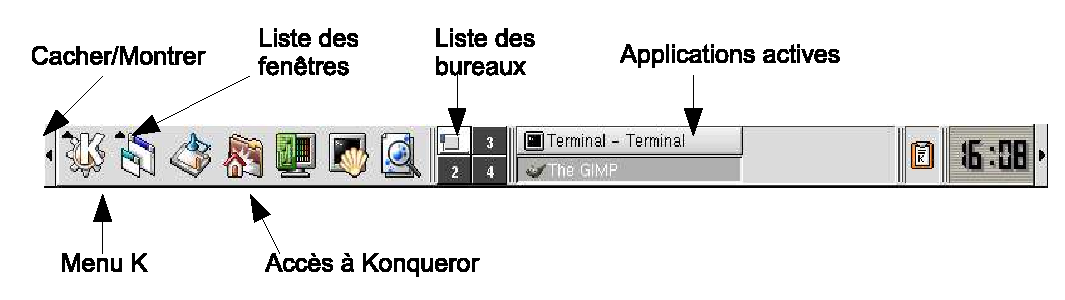
\includegraphics{img/kicker.eps}


\subsection{Gestions des fenêtres}

\subsubsection{Fenêtre active}

    La fenêtre active est la fenêtre vers laquelle est dirigée
    l'entrée clavier. En général, c'est la fenêtre qui est située par
    dessus les autres.  Pour rendre une fenêtre active, on peut
    utiliser la liste des fenêtres, la zone des applications actives
    (tableau de bord), ou bien cliquer (bouton gauche de la souris)
    sur la fenêtre.

\subsubsection{Outils de fenêtres}
    Certains outils sont disponibles pour améliorer la gestion des
    fenêtres. La partie supérieure de la fenêtre contient~: 

    \begin{itemize}
    \item {\bf Barre des titres} : affiche le titre de la fenêtre. Un
      double-clic sur la barre des titres permet de condenser la
      fenêtre.

    \item Bouton {\bf Fermer} : Ferme la fenêtre (et termine l'application
      s'il s'agit de la fenêtre principale de l'application).

    \item Bouton {\bf Maximiser/Réduire} : augmente ou réduit la taille de
      la fenêtre.
    \item Bouton {\bf Iconiser} : fait disparaître la fenêtre du
      bureau en la transférant vers la barre des
      fenêtres. Contrairement au bouton Fermer, l'application reste
      ouverte et peut etre reaffichée en cliquant sur la liste des
      fenêtres.


    \item Bouton {\bf Punaise} : permet de coller la fenêtre sur
      l'arrière-plan pour la faire apparaître sur tous les bureaux KDE
      (si la punaise n'est pas présente sur la barre de titre, faire
      un clic droit puis dans le menu Vers le bureau, choisir Tous les
      bureaux)

    \item En faisant un clic droit sur la barre de titre, on accède au
      menu de contrôle de la fenêtre qui reprend l'ensemble de ces
      options et permet, en plus, de déplacer une fenêtre d'un bureau
      à un autre.
    \end{itemize}



    \begin{center}
      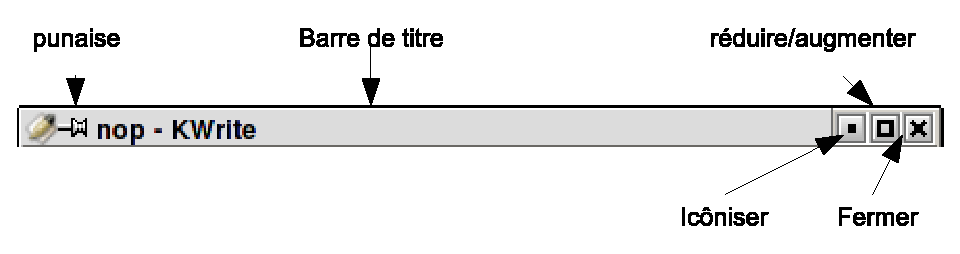
\includegraphics{img/barre.eps}
    \end{center}




\paragraph{Exercice d'application~:} l'éditeur de texte.

Le système KDE possède de nombreux éditeurs de texte simple
d'utilisation permettant de produire et de visualiser facilement des
documents.

\begin{itemize}
\item Chercher dans le menu K des éditeurs de texte simples comme {\tt
    kwrite} ou {\tt kate} et les lancer plusieurs fois.
\item Rendre ces fenêtres actives alternativement (à chaque fois,
  taper un texte au clavier).
\item Déplacer la fenêtre, changer la taille des fenêtres, déplacer
  une fenêtre dans un autre bureau, etc.
\item Clouer une des fenêtres de l'éditeur sur le bureau et entrer un
  texte. Se déplacer dans les autres bureaux pour observer ce qu'il se
  passe.
\end{itemize}


\section{SYSTÈME DE FICHIER LINUX/UNIX}

\subsection{Fichier et répertoire}

Un \emph{fichier} est ce qui contient l'information et un
\emph{répertoire} (ou \emph{dossier}) est l'endroit où sont rangés les
fichiers.

Sous Linux, cette notion de fichier est primordiale puisque 
les périphériques (disque dur, imprimante, lecteur de disquette, etc.)
du système sont considérés comme des répertoires.


Les répertoires sont organisés de façon hiérarchique, sous la forme
d'un arbre. La racine est le répertoire de plus haut niveau et est
symbolisée par le signe /. La figure \ref{fig:hierarchie} présente un
exemple d'organisation hiérarchique du système.



\begin{figure}[htbp]
  \centering
  \n{/}{
    \n{export}{\n{home}{\f{users}}}
    \f{root}
    \n{usr}{
      \n{bin}{
        \f{kate}
        \f{kwrite}}
      \f{lib}
      \n{local}{
        \f{bin}
        \f{doc}}}
    \n{media}{
      \f{cdrom}
      \f{floppy}
      \f{usbkey}}}
      
    
      
  \caption{Exemple de hiérarchie de répertoires et fichiers}
  \label{fig:hierarchie}
\end{figure}




Un fichier est localisé dans
une arborescence de répertoires à l'aide de son chemin. Exemple~: 
{\tt /usr/bin/kate} \emph{/home/licence} est le chemin menant au fichier
\emph{kate}. 



\subsection{Droits d'accès}
Le système Linux est multi-utilisateurs. Pour éviter les éventuels
conflits, les utilisateurs n'ont pas les mêmes droits d'accès sur
le système~:

\begin{itemize}
\item le simple utilisateur (vous) a des droits limités sur le
  système. Il possède un répertoire personnel
  ({\tt /export/home/users/licence/licence1/cp2i12009/TMP/c1pi-tmp-1})
  où il
  peut créer, modifier, effacer ses propres fichiers, et
  répertoires. Par contre, il n'a pas le droit d'aller modifier les
  fichiers des autres utilisateurs et les fichiers « sensibles » du
  système. Par exemple, il ne peut pas modifier les fichiers des
  répertoires {\tt /usr/bin}.  

\item le super-utilisateur (ou administrateur du système - « root » en
  VO) qui a tous les droits sur le système (y compris sur les
  répertoires des simples utilisateurs).
\end{itemize}



\subsection{Périphériques}
    Les périphériques (lecteur de disquette, lecteur de DVD mais aussi
    clavier, souris, écran...) sont considérés comme des répertoires
    particuliers. En particulier, le lecteur de clef usb est nommé
    {\tt /media/usbkey}. Pour copier un fichier sur une clef usb, il
    suffit de copier ce fichier dans ce répertoire.


\section{KONQUEROR : LE GESTIONNAIRE DE FICHIERS DE KDE}
\subsection{Préliminaire : utiliser une application et le copier-coller}
\subsubsection{Utiliser une application}

Il y a quatre façons de lancer des commandes à une application
(traitement de texte, tableur, jeu...)~: 
le menu, les boutons, le menu contextuel et les raccourcis clavier. Le
menu contextuel est un mini menu contenant les commandes les plus
utilisées. Il est affiché à l'aide d'un clic-droit sur la souris. 
Si dans un premier temps, vous préférerez vous perdre dans
l'arborescence des menus, l'expérience aidant, vous connaîtrez
sûrement quelques raccourcis clavier. 

\subsubsection{Copier-coller}
La notion importante à comprendre ici est celle du Copier-Coller. Ce
principe se retrouve dans la plupart les applications permettant de
manipuler des objets tels que les chaînes de caractères, les fichiers,
les répertoires, les images, etc... 

\begin{itemize}
\item \emph{Copier} signifie réaliser une copie de l'objet sélectionné
  dans un espace réservé de l'ordinateur, appelé presse-papier.
\item \emph{Couper} effectue la même commande que Copier, à la différence que
  l'objet coupé est supprimé.
\item \emph{Coller} signifie prendre l'objet qui est dans cet espace réservé
  (s'il existe) et le recopier.
\end{itemize}


\begin{center}
  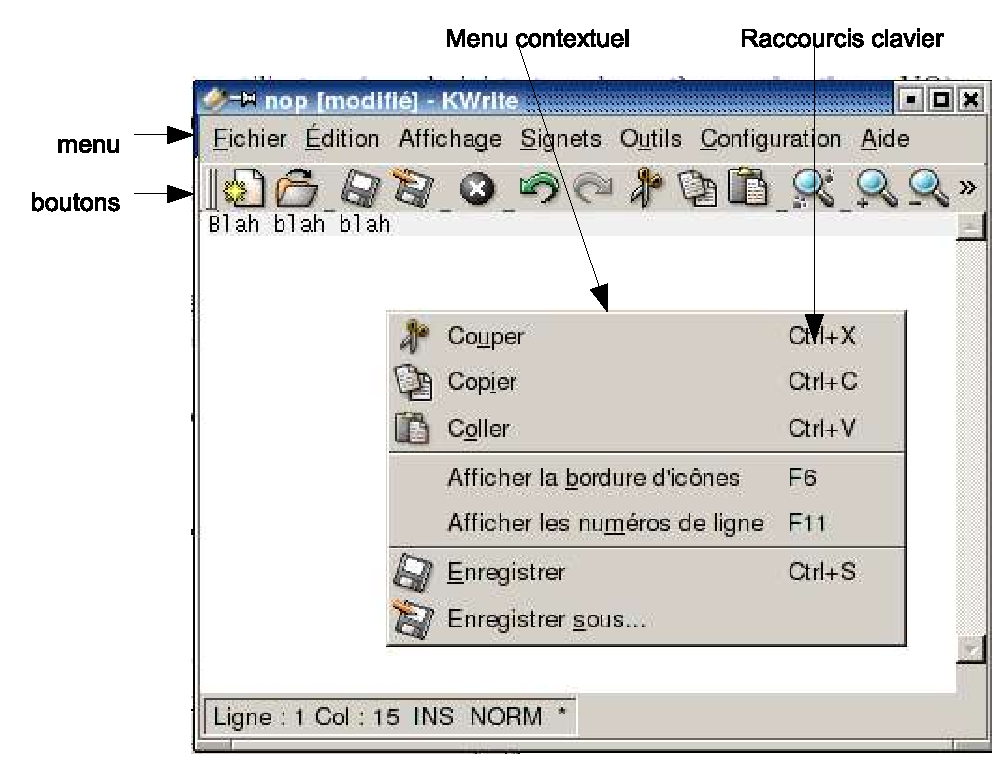
\includegraphics{img/kwrite.eps}
\end{center}

Ces options sont disponibles soit dans la barre des icônes de
l'éditeur de texte soit dans le menu Édition.

Ouvrir l'éditeur de texte et taper le texte suivant (en respectant le
saut de ligne)~:

\begin{verbatim}
Blah blah blah.
Bof.
\end{verbatim}

\begin{enumerate}
\item Sélectionner le texte entier (en maintenant le bouton
  gauche de la souris appuyé tout en déplaçant celle-ci sur le
  texte). Une fois le texte sélectionné (le texte sélectionné apparaît
  en surbrillance), copier ce texte. Dé-sélectionner le texte et
  appliquer la commande Coller. Le morceau préalablement copié
  s'insère alors à la position courante du curseur.

\item Ouvrir un second éditeur de texte. Appliquer la commande Coller,
  le texte doit alors s'insérer dans le nouvel éditeur. On peut ainsi
  faire du copier-coller entre plusieurs applications.

\item Sauvegarder ensuite les deux textes, sous deux noms différents,
  le premier sous le nom {\tt blah1.jpg} et le second sous le nom
  {\tt blah2.txt} dans votre dossier personnel.
\end{enumerate}



\subsection{Le gestionnaire de fichier}
Le navigateur appelé Konqueror permet de visualiser le contenu d'un
répertoire précis. Pour le lancer, utilisez le menu K ou cliquez sur
la petite maison située sur votre bureau. 

Le navigateur se présente de la façon suivante (de haut en bas):
\begin{itemize}
\item la barre des menus (Document, édition, ...) ;
\item la barre d'outils (ou barre des icônes) ;
\item la barre d'emplacement : affiche le chemin absolu du répertoire
  courant ;
\item enfin, la zone de contenu.
\end{itemize}


\begin{center}
  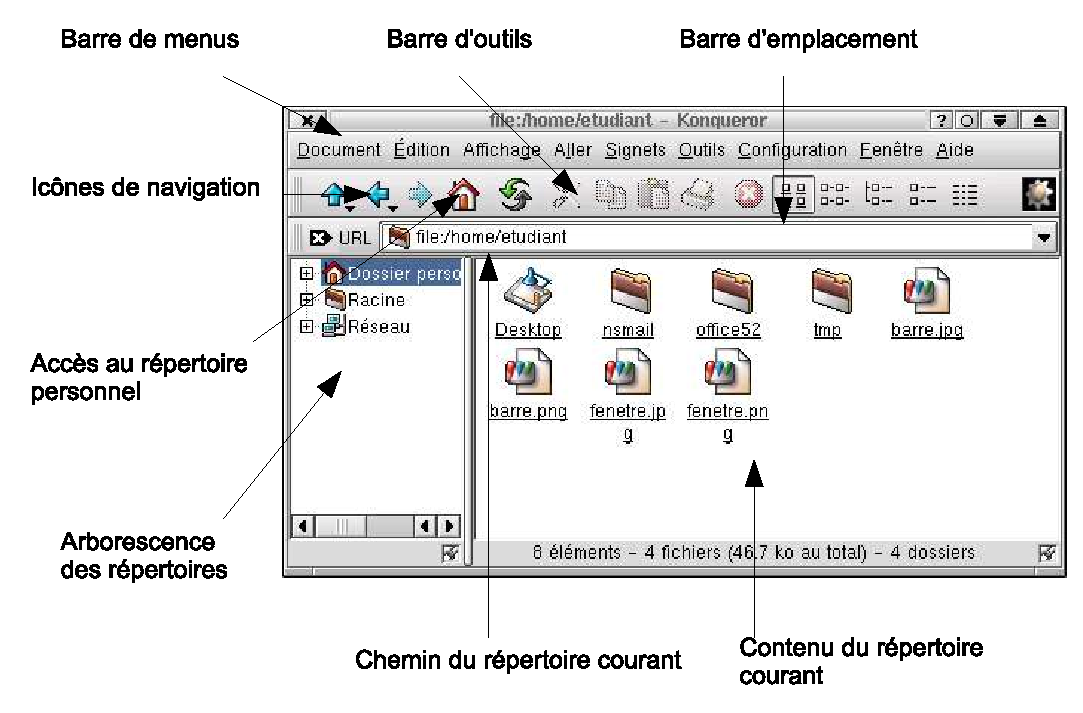
\includegraphics{img/konqueror.eps}
\end{center}


\subsubsection{Barre des menus}

Le menu \emph{Édition} permet de faire des opérations courantes sur le
contenu des répertoires ou sur des fichiers (création, etc.). On
retrouve ici le \emph{Copier-Coller} que l'on peut appliquer sur des fichiers
ou des répertoires. 

Le menu \emph{Affichage} propose diverses options sur
l'affichage. Ainsi, en sélectionnant l'option \emph{Type d'affichage},
puis \emph{Liste détaillée}, vous obtenez des informations détaillées
sur chacun des fichiers du répertoire courant (le type de contenu,
leur taille, leur date de modification, etc.).

Le menu \emph{Fenêtre}, puis \emph{Afficher panneau de navigation},
vous permet d'obtenir une sous-fenêtre supplémentaire sur la
gauche. Cliquez alors sur l'icône \emph{Dossier racine} de cette
sous-fenêtre (utilisez les bulles d'aide pour le trouver) et
l'ensemble de l'arborescence du système s'affiche dans la zone de
contenu.

Le menu \emph{Aller} contient des raccourcis pratiques.

Le menu \emph{Signets} propose une liste... de signets. Un signet (ou
bookmark en VO) est un lien vers une page Web, vers un fichier ou
répertoire local. Vous pouvez définir des signets pour accéder 
facilement aux répertoires de votre choix.



\subsubsection{Barre d'outils}
   Cette barre contient des icônes facilitant la navigation en
   particulier (de gauche à droite)~:
 
   \begin{itemize}
   \item la flèche vers le haut qui permet de remonter d'un cran
     dans l'arborescence (par exemple, on passe du répertoire
     \emph{/usr/bin} au répertoire \emph{/usr})

   \item la flèche vers la gauche qui permet de revenir en arrière
     dans l'historique des répertoires que l'on a parcouru.

   \item la flèche vers la droite qui permet de repartir vers l'avant
     dans l'historique des répertoires parcourus (il faut bien sûr
     avoir utilisé la flèche gauche auparavant). 

   \item La \emph{maison} permet de revenir au répertoire personnel.

   \item on retrouve ensuite les icônes de Copier-Coller.
   \end{itemize}


\subsubsection{Travail sur les fichiers}

\paragraph{Sélection\\}
Le fait de cliquer avec le bouton gauche de la souris sur un fichier
sélectionne le fichier. Si l'on désire ouvrir le fichier (ou le
répertoire), il faut double-cliquer.

\paragraph{Déplacement de fichier\\}
Une fois le fichier (ou répertoire) sélectionné, on peut le copier,
le déplacer, l'effacer. KDE, comme d'autres systèmes de gestion de
fenêtres, adopte le principe du Glisser-Déposer \emph{drag and
  drop}. On peut ainsi copier, déplacer ou lier (i.e. créer un
raccourci vers un fichier) des fichiers ou des répertoires uniquement
avec la souris par déplacement de fichiers sélectionnés.

Un lien est un pointeur vers un fichier ou un répertoire. Ce n'est pas
une copie du fichier ou du répértoire. Cela permet d'obtenir des
raccourcis vers ce fichier. A la différence d'un signet, le lien se
comporte comme un fichier, et peut être copié-collé.

\paragraph{Ouverture des fichiers\\}
Konqueror reconnaît par défaut certains types de fichiers~: il est
possible d'ouvrir ces fichiers par un double-clic sur le bouton gauche
de la souris sur ce fichier. Ces types de fichiers répondent plus ou
moins à la norme MIME qui vise à standardiser les différents types de
fichiers. Par exemple, dans votre répertoire personnel, un clic sur
le fichier {\tt blah2.txt} ouvre le fichier~: le type du fichier
dépend en partie de l'extension de ce fichier. Par exemple, si on
clique sur le fichier {\tt blah1.jpg}, Konqueror considère que ce
dernier est une image et essaye de l'ouvrir en tant que tel (ce qui
n'est pas possible). 

\subsection{Gestion de la corbeille}
   Sous Linux, la suppression des fichiers est DÉFINITIVE, sans aucun
   moyen de les récupérer. Il est donc prudent de réfléchir à deux
   fois avant d'effacer un fichier. Sous KDE, les développeurs ont mis
   en place une corbeille, une zone temporaire où l'on met les
   fichiers que l'on veut supprimer. Si l'on décide finalement de ne
   pas supprimer un fichier, il suffit alors d'ouvrir cette corbeille
   (présente sur votre bureau) et de copier le fichier à
   récupérer. Pratiquement, la corbeille correspond à un répertoire~:
   mettre un fichier à la corbeille revient à déplacer ce fichier dans
   le répertoire de la corbeille ({\tt <votre répertoire
     personnel>/Desktop/Corbeille}). 



\subsection{Exercices d'application}
\subsubsection{Manipulation des fichiers et des répertoires}

\begin{itemize}
\item Créer, avec le navigateur,
  l'arborescence suivante à partir de votre répertoire personnel; 

  \begin{center}
    {\tt
      \n{info}{
        \n{tp1}{
          \f{tp11}
          \f{tp12}}
        \f{tp2}}
    } 
  \end{center}
  

\item Déplacer les fichiers
  {\tt blah2.txt} et {\tt blah1.jpg} dans le
  répertoire {\tt tp1} ; 

\item Copier le fichier {\tt blah1.jpg} dans le répertoire
  {\tt tp11}.
  
\item Double-cliquer sur le fichier
  {\tt blah1.jpg} (celui de tp11). Que se
  passe-t-il ?

\item Renommer ce fichier en
  {blah1.txt}. Double-cliquer dessus. Que se
  passe-t-il maintenant~? Que peut-on en conclure~?

\item Effacer le fichier {\tt blah1.txt}.

\item Mettre les répertoires {\tt tp11} et {\tt tp12} à la
  corbeille.

\item Effacer ensuite le contenu de la
  corbeille.
\end{itemize}

Finalement, déplacez-vous dans le répertoire {\tt
  /export/home/users/Enseignants/rozenknop/pub/ cp2i/TP01/sujets} et
double-cliquez sur le sujet de TP adéquat pour passer à la suite.

\end{document}
